
\begin{intro}{一首音乐—逻辑的奉献}

\noindent 作者:

普鲁士的国王腓德烈大帝于1740年即位。虽然他主要以军事上的精明而著称于世,但是对思想和精神方面的东西也非常热衷。他在波茨坦的宫廷是十八世纪欧洲知识界活动的主要中心之一。著名数学家欧拉在那里住过二十五年。还有许多别的数学家、科学家以及哲学家——包括伏尔泰和拉·梅特利在内,他们的一些最有影响的作品就是在那里写出来的。

但是,腓德烈的真正爱好是音乐。他是个热心的长笛手和作曲家。他的一些作品甚至到现在还被演奏。腓德烈是最早认识到新发明的“弱强琴”[piano-forte]\lnote{(即钢琴[piano]的原名)}优点的艺术保护人之一。十八世纪前半叶,羽管键琴(又称拨弦古钢琴)经过改造发展成为钢琴。羽管键琴的缺点是,乐曲只能以同一响度奏出,而无法把一个音符弹得比它前后的音符更响些。“弱强琴”——正像这一名称本身所暗示的那样——弥补了这一缺陷。在意大利,巴托罗米欧·克里斯托弗制造了第一架这种钢琴。以后,“弱强琴”这个概念就从意大利广泛地传播开了。第一流的德国管风琴制造家哥特弗雷德·希尔伯曼当时致力于制造一架“完备”的弱强琴。腓德烈大帝无疑是他这一工作的最大支持者——据说这位国王拥有的希尔伯曼钢琴达十五架之多!

\begin{figure}
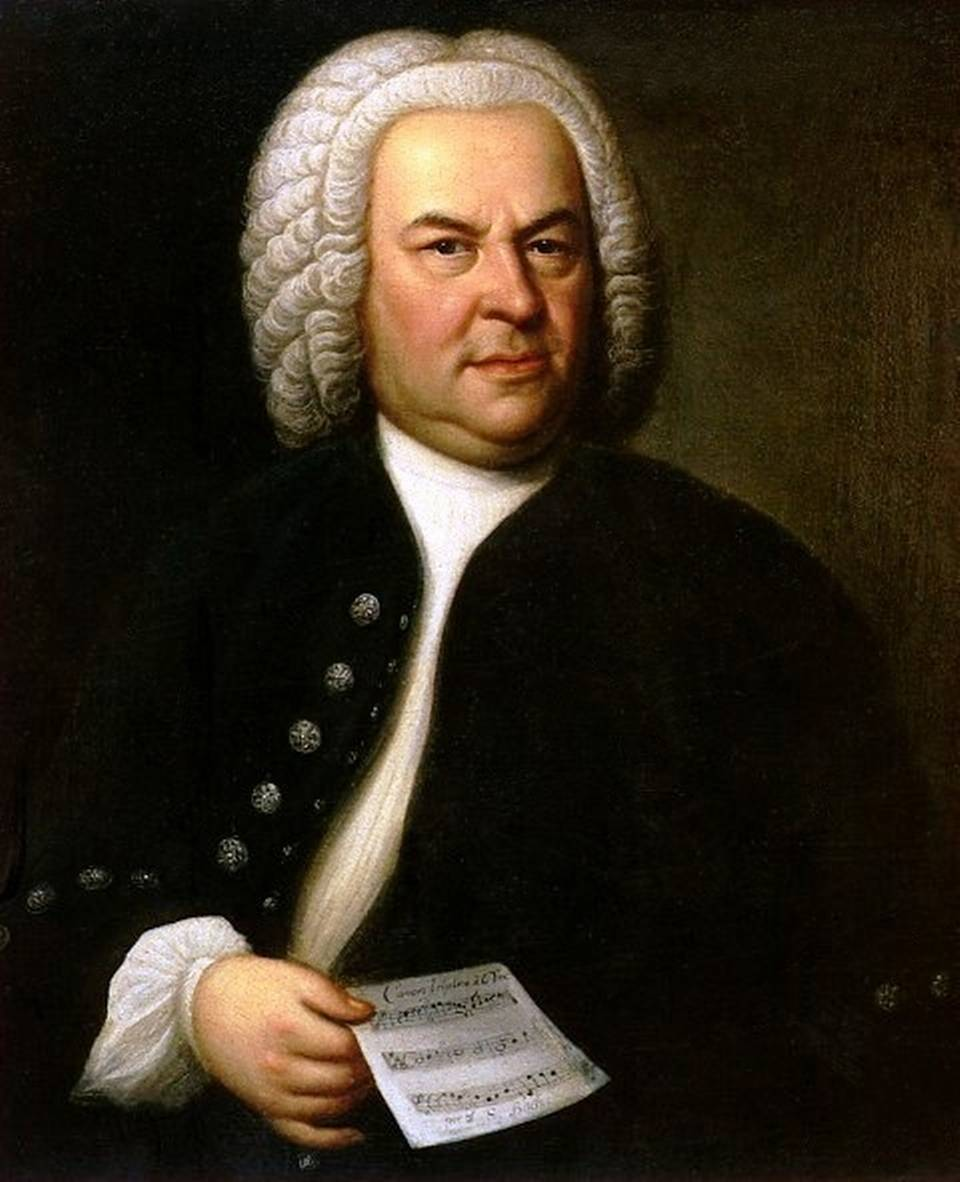
\includegraphics{img_001.jpg}
\caption[约翰·塞巴斯第安·巴赫,艾利亚斯·哥特利伯·豪斯曼作。]
  {约翰·塞巴斯第安·巴赫在1748年。取自艾利亚斯·哥特利伯·豪斯曼的一幅油画。}
\end{figure}

\section{巴赫}

腓德烈大帝不仅是个钢琴爱好者,而且也是管风琴师兼作曲家约·塞·巴赫的崇拜者。这位巴赫的作品当时是颇有争议的。有些人认为它们是“浮华而混乱的”,有些人则声称他的作品是无与伦比的杰作。但是没人对于巴赫在管风琴上即兴演奏的能力有什么异议。在那个时代,作一名管风琴家不仅意味着能演奏,并且还要能即兴创作,而巴赫就是以他那非凡的即兴创作能力遐迩闻名的(如果想了解有关巴赫即兴创作的一些趣闻轶事,请看汉·西·大卫和阿·曼德尔著的《巴赫读本》一书)。

1747年,巴赫六十二岁,他的名声和他的一个儿子同时到达了波茨坦。事实上,卡尔·菲利普·埃玛努厄尔·巴赫\note{译者注:约·塞·巴赫的第三个儿子。}是腓德烈国王宫廷合唱队的指挥。多年来,这位国王一直暗示菲利普·埃玛努厄尔,他非常希望老巴赫能来拜访他;但是,这一愿望一直还没能实现。腓德烈尤其渴望巴赫能试一下希尔伯曼制造的新钢琴,当时他正确地预见到这种乐器将会成为席卷音乐界的一股巨大的新潮。

\begin{figure}[b]
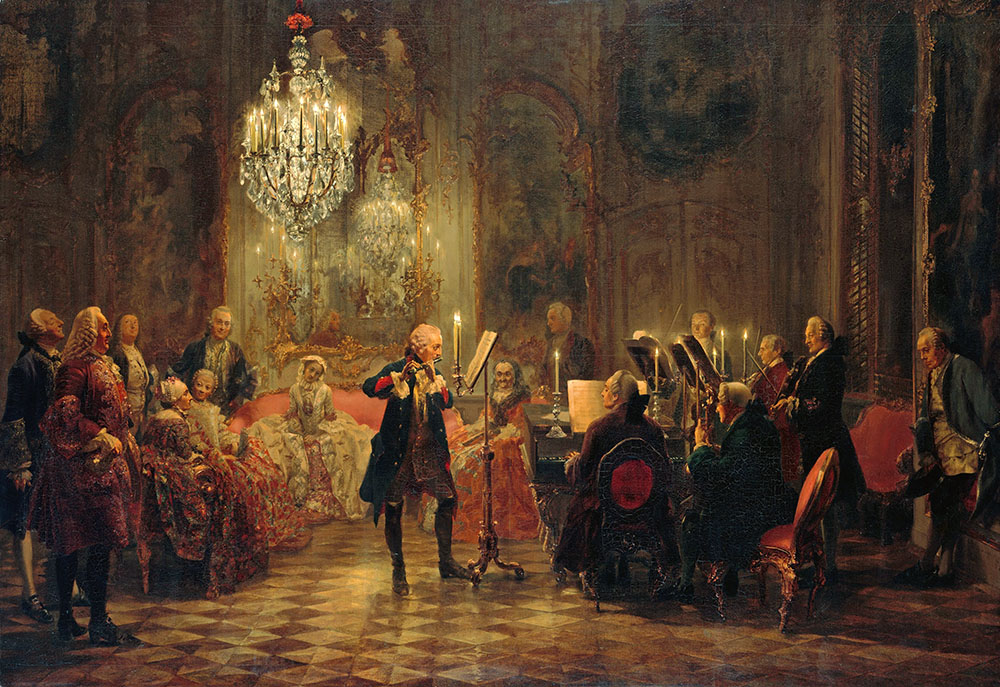
\includegraphics{img_002.jpg}
\caption[无忧宫中的长笛音乐会,阿道夫·封·门采尔作。]
  {无忧宫中的长笛音乐会,阿道夫·封·门采尔\pnum{1852}。}
\end{figure}

腓德烈惯常在晚上举行宫廷室内乐音乐会。他自己常常喜欢担任长笛协奏曲中的独奏。\fig{2}就是一幅表现这样一个晚会的油画,这幅画出自德国画家阿道夫·封·门采尔之手,门采尔在十九世纪初画了一系列展示腓德烈大帝生活的油画。弹羽管键琴的是卡·菲·伊·巴赫,右边最远处的那个人物是国王的长笛教师约辛·昆茨。他是唯一有权给国王的长笛演奏挑毛病的人。1747年5月的一个晚上,一位意想不到的客人来访了。巴赫最早的传记的作家之一约翰·尼古拉·福凯尔讲述了下面这个故事:

\begin{quote}
一天晚上,正当他把长笛准备好,他的乐师们也都集合起来的时候,一位官员呈递给他一份来访的陌生人的名单。他手里拿着长笛,看了一眼名单,随即便转向聚在一起的乐师们兴奋地说:“先生们,老巴赫来了。”长笛被放在了一边。老巴赫——当时落脚在他儿子的家里——立即被召进宫里。威廉·弗里德曼\note{译者注:约·塞·巴赫的长子。}陪伴着他父亲,这段故事就是他给我讲的。现在想起他给我讲这段故事时的那副神态,仍然让我感到很愉快。见面时说一段冗长的恭维话是那个时代的一种风尚。巴赫在初次拜谒这样一位伟大的国王时,一定说了许多致歉的话,因为国王甚至没有给他时间让他把行装换成演奏时穿的黑礼服。我在此不准备复述那些致歉的话,而只是指出,据威廉·弗里德曼讲,国王与道歉者之间进行了一次很客套的对话。
\end{quote}

\begin{quote}
但比这更重要的是国王取消了那天晚上的音乐会,转而邀请巴赫——当时已被称做老巴赫——试一试他的那些希尔伯曼制造的钢琴,这些钢琴摆在宫中几个房间里。\lnote{(福凯尔在这里加了一个注:“国王非常喜欢弗莱堡的希尔伯曼制造的钢琴,并且决定全部买下。他一共收集了十五架。我听说现在它们被摆在皇宫的各个角落里,都已不能使用了。”)}乐师们跟着国王从一个房间走到另一个房间,每到一处巴赫都被邀请试试那些钢琴,进行亳无事先准备的即兴演奏。这样弹了一会儿之后,他要求国王给他一个赋格主题,以便在没有任何准备的情况下立即演奏它。国王非常欣赏巴赫即兴演奏这一主题的那种高超的方式。他表示希望能听到一首有六个非自由声部的赋格曲。这大概是想了解这种技巧能发挥到什么程度。但是因为并非任何主题都能适合于这种丰满的和声,所以巴赫自己选择了一个主题,而且立即以他演奏国王的主题时的那种庄严和高超的方式,演奏了他自己的这支主题,这使得所有在场的人惊讶不已。国王陛下还想听他演奏管风琴。于是翌日,巴赫像前一天演奏希尔伯曼钢琴一样,弹奏了波茨坦所有的管风琴。回到莱比锡以后,他用三部和六部的形式为国王的那个主题谱了曲,另外还加上了几段以严格的卡农形式同那一主题相对应的经过句,将它冠以“Musikalisches Opfer”\lnote{(《音乐的奉献》)}的标题付梓,并把它献给了那个出题者。\note{大卫和曼德尔,《巴赫读本》,第305--306页。}
\end{quote}

巴赫把一本《音乐的奉献》连同一封致献信函一起呈给了国王。这封信仅就其文体来说,就是饶有兴趣的——相当谦恭和谄谀。用现代的眼光来看,这封信似乎带点滑稽味道。这大概可以使人想象巴赫初见国王时那番致歉的风格。\note{大卫和曼德尔,《巴赫读本》,第179页。}
\begin{quote}
最仁慈之国王陛下:

微臣在此最卑微地呈给陛下一曲音乐之奉献。其最高贵部分出自陛下圣手。初,微臣荣造波茨坦,陛下曾纡尊为臣在钢琴上奏一赋格主题,且广施恩泽,令微臣于陛下御前将其敷演成章,如此弘恩殊宠使臣诚惶诚恐,得意感戴,念念不忘。遵从陛下御旨乃臣最谦卑之职分。然微臣旋念,猝然无备便措手此任,恐有负于此一如此杰出之主题。故微臣旋即立意:誓将此国王主题充分发挥,并使之昭彰于世。此誓言今已化为现实。就光耀一位于有关战争与和平之所有学问中——尤以音乐为殊——均具有令人人尊慕之伟大与权威之君王而言,此一无可挑剔之创意实乃无与伦比。臣斗胆妄加如下最谦卑之请求:愿陛下纡尊恩纳这一微薄之功作,以使其由于您之惠纳而得以抬高,并请求陛下续垂恩典。

\begin{signature}[l]
陛下\\
\qquad 您最卑微恭顺之仆人:\\
\ziju{.5}\qquad\qquad 作者
\end{signature}
\nopagebreak\begin{tabular}[b]{c}
1747年7月7日于\\
莱比锡
\end{tabular}
\end{quote}

\begin{figure}
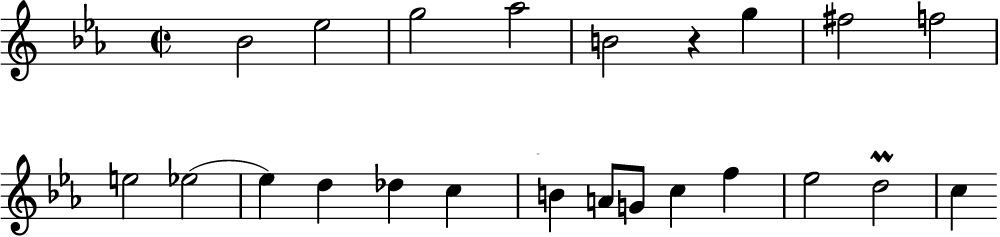
\includegraphics{img_003.png}
\caption{国王主题。}
\end{figure}

过了二十七年,那时巴赫已故去二十四年了,一位名叫哥特弗雷德·封·施维腾的男爵(顺便提一句,福凯尔的巴赫传记以及贝多芬的《第一交响曲》都是题献给他的)同腓德烈大帝有过一次交谈,关于那次谈话的情况他是这样记述的:

\begin{quote}
他\lnote{(腓德烈)}跟我谈到了音乐和一位名叫巴赫的了不起的管风琴师,他在柏林曾经住过一段时间。这位艺术家\lnote{(威廉·弗里德曼·巴赫)}在和声知识的深度和演奏能力方面所具有的天才超过我听到过或能想象到的任何人。但那些认识他父亲的人说,他父亲甚至更了不起。国王也持有这样的看法。为了向我证明这一点,他高声唱起了他给老巴赫出的那个半音阶的赋格主题。当时巴赫用这个主题当场敷奏了一首开始有四个声部,然后是五个声部,最后到八个声部的赋格曲。\note{大卫和曼德尔,《巴赫读本》,第260页。}
\end{quote}

当然,我们无从知道究竟是腓德烈国王还是施维腾男爵把故事夸张到了耸人听闻的地步。但它说明了在那个时期,有关巴赫的传说是多么厉害。要想理解有六个声部的赋格是多么耸人听闻,你应该知道巴赫的整部《平均律钢琴曲集》中有四十八首前奏曲和赋格,其中多达五个声部的赋格只有两首,六个声部的赋格则根本没有!我们可以把即兴创作六个声部的赋格比做同时下六十盘盲棋,而且全部要下赢。即兴创作有八个声部的赋格则的确非人力所能及。

在巴赫献给腓德烈国王的那本乐谱的扉页上有这样的题辞:
\begin{figure}[H]

\includegraphics{img_004.png}
\caption[巴赫的字首字母组合“RICERCAR”。]
  {奉旨承诏,将歌曲及余部以卡农技巧予以解决。}
\end{figure}
巴赫在这里使用卡农(canonic)这个词语意双关,它不仅有“用卡农”(with canon)的意思,还包含着“用可能有的最好方式”的意思。这句题辞的每个词的首字母排在一起是
\begin{center}
RICERCAR
\end{center}
——这是个意大利词,意思是“探求”。《音乐的奉献》中确实有许多东西需要探求。它包括一首三声部的赋格,一首六声部的赋格,十首卡农曲和一首三重奏鸣曲。音乐专家们认为,那首三部赋格一定和巴赫为腓德烈国王即兴创作的那一首基本相同。那首六部赋格是巴赫最复杂的作品之一,其主题自然是那个国王主题。该主题——如\fig{3}所示——非常复杂,它的节奏是不规则的,又是高度半音化的(这也就是说,里面充满了该曲的调外音)。对一般的音乐家来说,甚至根据它来写一首好的二部赋格都不是件容易的事!

两首赋格都题有“Ricercar”,而不是“Fuga”的字样。这是“探求”[ricercar]一词的另一个意思。“ricercar”其实就是现在被称为“赋格”[fugue]的这种曲式的原名。到了巴赫那个时代,“赋格”[fugue]一词(或拉丁文和意大利文的fuga)已是标准用语了,“ricercar”这个词仍然存在,但转义为专指一种艰深复杂的赋格,中文叫做“无插入赋格”。也许在一般人听起来,这个词过于咬文嚼字了。现代英语中还保留着一个与之类似的说法:“recherché”,其字面意思是“找出”,但同样具有深奥或学究的味道。

三重奏鸣曲将人们从严肃的赋格和卡农中愉快地解脱出来。因为它的旋律甜美动听,几乎可以应之起舞。然而,它主要也是建立在那么半音化和那么庄严威峻的国王主题上的。巴赫能用这样的主题创作出如此动听的间奏曲真可谓是奇迹了。

《音乐的奉献》中那十首卡农可被列入巴赫所写过的最复杂的卡农之中。然而非常奇怪的是,巴赫从未把它们完整地写出来。他这样做是有意的。这些卡农是作为难题向腓德烈王呈上的。当时很流行的一种音乐游戏是,出一个主题并给出或多或少的巧妙暗示,让另一个人去“发现”建立在那个主题上的卡农。为了了解这是如何可能的,必须得懂得一些关于卡农的知识。

\section{卡农和赋格}

卡农的基本点是一个单一的主题与它自己相伴而奏。由加入的各个不同声部分别唱出主题的“副本”。但做这种事可以有许多种方式。卡农中最简单的是轮唱,像《保卫黄河》,第一个声部先唱出主题,相隔规定的某段时间之后,这一主题的“副本”在完全一样的调上进入。在这第二个声部进行到规定的同样长的时间之后,第三个声部进入,唱出这个主题,以此类推。对大部分的主题来说,这样演唱是无法与它本身相和谐的。为了使一个主题能成为一支卡农的主题,它的每个音符必须能起两种(三种,或四种)作用:首先它得是旋律的一部分,其次它必须是这同一旋律的和声的一个部分。比如说,在包含有三个卡农式声部的曲子里,主题的每一个音符除了要构成曲调,还必须在两种不同的方式上构成和声。这样,在卡农曲中,每个音符都有着一个以上的音乐意义,而听者的耳朵和大脑根据前后的音调自动地领会其确切的意义。

当然还有更复杂的卡农。按由简入繁的顺序,第一种更复杂的卡农是:主题的种种“副本”不仅在时间上,而且在音高上互相交错。也就是说,第一声部可能是在C调上唱出主题,同第一声部相交错的第二声部可能是在比C调高五度的G调上唱出同一主题。与前两个声部相交错的第三声部可能在比G调高五度的D调上唱出,以此类推。下一种更复杂的卡农是:各个声部的速度不同,比如说,第二个声部的速度可能是第一声部的二倍或一半。前者叫做减值,后者叫做增值(因为主题好像是在收缩或者扩展)。

这还不算完。卡农构成中下一个更复杂的阶段是主题转位,意思是产生这样一个旋律,每当原来的主题跳上时,它就跳下,两者所越过的半音数目相同。这是种相当奇特的旋律转换,但是,如果一个人听过很多转位的主题,就会觉得这种事挺自然了。巴赫就特别喜欢转位,并经常在他的作品中使用——《音乐的奉献》也不例外。作为转位的一个简单例子,可以试着唱唱《好国王温赛拉斯》[\bn{Good King Wenceslas}]这支曲子。当它的原主题和转位主题一起唱出时,高低相差八度,前后相差两拍,这就是一支相当悦耳的卡农曲了。最后,这些“副本”中最玄奥的是逆行——主题依一定时间从后往前奏出。使用了这种技巧的卡农,俗称为“螃蟹卡农”,这是因为螃蟹那奇特的运动方式。不用说,巴赫《音乐的奉献》中也包含有一支螃蟹卡农。注意,不论是哪一种“副本”,都保持有原主题的所有信息,也就是说,从任何一种副本中都可以完全恢复原主题。这种保存信息的转换经常被称作同构。在本书中,我们将经常谈到同构。

有时候需要放松这种很严格的卡农形式。一种办法是允许稍稍偏离完全的反复,以取得更流畅的和声。也有的卡农有“自由”声部——这种声部不使用该卡农的主题,只是和该卡农中的各个声部和谐一致。

《音乐的奉献》中的每一支卡农都以国王主题的某个变奏作为自己的主题。上面所说的每一种使卡农复杂化的手法在《音乐的奉献》中都被充分使用了。事实上,这些方法有的时候是结合起来使用的。比如,其中有一首三部卡农被称做《反向增值的卡农》。它的中间声部是自由声部(实际上,它唱的是国王主题),而其它两个声部用增值和转位的手法以卡农形式在其上下跳跃。另外一个声部则仅仅是用一句神秘的“quaerendo invenietis”(“觅之,自有所获”)标示着。所有的卡农谜题都解决了,典范的解决是由巴赫的一个学生约翰·菲利普·科恩伯格给出的。但是人们仍然可以设想还有更多的解决有待发现呢!

我还应该简单解释一下什么是赋格。赋格在下述这一点上像卡农一样:它通常也是建立在一个主题上,以不同的声部、不同的调子、偶尔也用不同的速度或上下颠倒或从后往前地进行演奏。然而,赋格的概念远不如卡农那么严格,因而允许有更多的情感或艺术的表现。赋格的识别标志的是它的开始方式:单独的一个声部唱出它的主题,唱完后,第二个声部或移高五度或降低四度进入。与此同时,第一个声部继续唱“对应主题”,也叫第二主题,用来在节奏、和声、及旋律方面与主题形成对比。每个声部依次唱出主题,常常是另一个声部伴唱对应主题,其它的声部所起的作用随作曲家的想象而定。当所有的声部都“到齐”了,就不再有什么规则了。当然,还是有一些标准的手法,但它没有严格到只能够按照某个公式去创作赋格。《音乐的奉献》中的两首赋格曲就是杰出例子,它们决不可能“照公式创作出来”。这两首曲子都具有远比赋格的性质更为深刻的东西。

总的来说,《音乐的奉献》是能代表巴赫在对位法方面最高成就的作品之一。它本身就是一部大型的、高度理智化的赋格,其中许多概念和形式彼此交织,游戏式的双重意义和微妙的影射随处可见。这是一部令人百听不厌的人类智能的优美绝伦的创作(汉·西·大卫在《巴赫的〈音乐的奉献〉》一书中对整个作品做了精彩的描述)。

\section{无穷升高的卡农}

在《音乐的奉献》中有一首极不寻常的卡农,只标着“Canon per Tonos”(经由种种调性的卡农)这么三个词。它有三个声部,最高声部是国王主题的一个变奏,下面两个声部则提供了一个建立在第二主题之上的卡农化的和声。这两个声部中较低的那个声部用C小调(这也是整部卡农的调)唱出主题,而较高的那个则在差五度之上唱同一主题。这首卡农与其它卡农的不同之处在于,当它结束时——或者不如说似乎要结束时——已不再是C小调而是D小调了。巴赫在听众的鼻子底下转了调。而且这一结构使这个“结尾”很通顺地与开头联接起来。这样我们可以重复这一过程并在E调上回到开头。这些连续的变调带着听众不断上升到越来越遥远的调区,因此听了几段之后,听众会以为他要无休止地远离开始的调子了。然而在整整六次这样的变调之后,原来的C小调又魔术般地恢复了!所有的声部都恰好比原来高八度。在这里整部曲子可以以符合音乐规则的方式终止。人们猜想,这就是巴赫的意图。但是巴赫很明确地留下了一个暗示,说这一过程可以无休止地进行下去。也许这就是为什么他在边空上写下了“转调升高,国王的荣耀也升高。”为强调它潜在的无穷性质,我喜欢把它叫做“无穷升高的卡农”。

在这部卡农中,巴赫给了我们有关“怪圈”这一概念的第一个例子。所谓“怪圈”现象,就是当我们向上(或向下)穿过某种层次系统中的(这里,系统是音乐的调子)一些层次时,会意外地发现我们正好回到了我们开始的地方。有时我用“缠结的层次结构”这个词来形容出现怪圈的系统。在我们后面的讨论中,怪圈这一主题将一再出现。有时候它是隐蔽的,有时候则会公开露面,有的时候它端端正正,有的时候则上下颠倒,或者前后错位。“觅之,自有所获”,这便是我给读者的建议。

\section{艾舍尔}

在我看来,把怪圈概念最优美最强烈地视觉化了的人是荷兰版画家毛·康·艾舍尔(1898--1972)。艾舍尔创作了一些迄今以来最富于智能启发力的杰作。他的许多作品都源于悖论、幻觉或双重意义。数学家属于艾舍尔作品的第一批崇拜者,这是不难理解的,因为他的画经常是建立在对称或模式等等这类数学原理上的。但是一幅典型的艾舍尔作品所含的内容远不仅是对称或模式。在他的作品里常常有一个化入艺术形式里的潜在概念。具体点说,怪圈就是艾舍尔画中最常出现的主题之一。例如石版画《瀑布》(\fig{5})。请把它的六步无终止下降圈和《经由种种调性的卡农》的六步无终止上升圈做一下比较。视觉上的这种相似性是很值得注意的。巴赫和艾舍尔用两个不同的“调子”——音乐和美术——演奏着同一个主题。

\begin{sidewaysfigure}
\begin{floatrow}
\figurebox{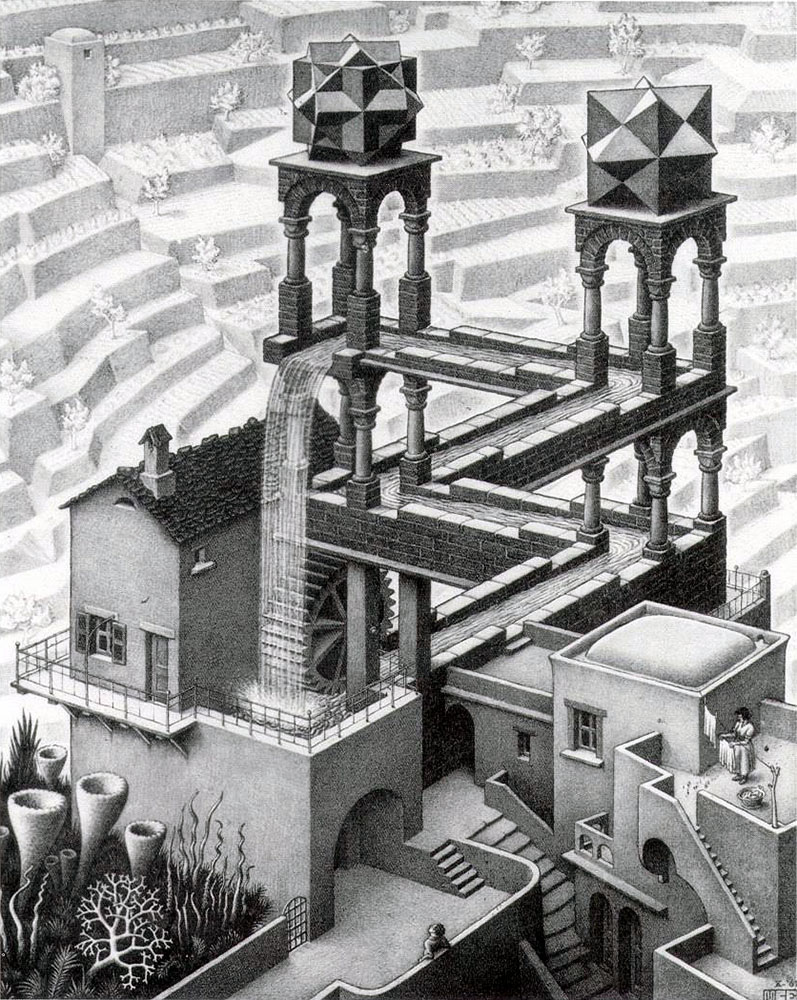
\includegraphics{img_005.jpg}}
          {\caption[瀑布,艾舍尔作。]{瀑布,艾舍尔作(石版画,1961)。}}
\figurebox{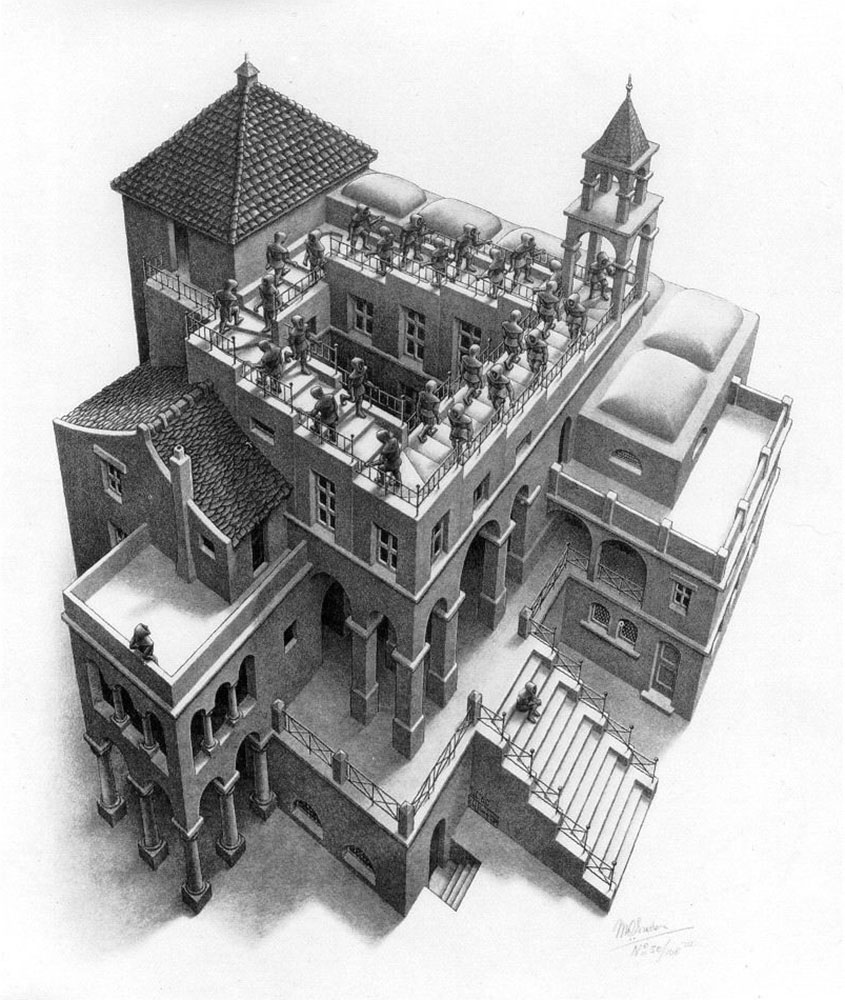
\includegraphics{img_006.jpg}}
          {\caption[上升与下降,艾舍尔作。]{上升与下降,艾舍尔作(石版画)。}}
\end{floatrow}
\end{sidewaysfigure}

艾舍尔用了几种不同方式来表现怪圈,它们可以依照圈的紧凑程度排列起来。石版画《上升与下降》(\fig{6})中,修士们永无休止地转着圈子。这是最松散的一幅,因为在回到原出发点以前要经过许多阶段。《瀑布》中的圈就要紧凑一些,正如我们所看到的,它只有六个分立的阶段。你可能会觉得“阶段”这个概念有些模糊,比如,在《上升与下降》这幅画中,把它看成有四段(楼梯)和把它看成有四十五级(台阶)不是一样容易吗?的确,在如何数层次这一问题上,历来就有些模糊,这个问题不仅仅存在于艾舍尔的画中,也存在于多层次的层次系统中。以后我们会对这种模糊有更深入的理解。现在,我们还是别离题太远。《画手》给我们提供了一个更紧凑的圈(\fig{135}),这幅画中的每一只手都在画另一只手:这是个只包含两个阶段的怪圈。最后,我们遇到了所有怪圈中最紧凑的:它表现在《画廊》(\fig{142})这幅画中:这是一幅包含其自身的画。是否能说它是一幅描绘一座包含其自身的画廊的画?或者说它是描绘了一个包含其自身的城市的画?还是说它是一个包含了自己的年青人?(顺便提一句,《上升与下降》及《瀑布》中所运用的那种视力幻觉法不是艾舍尔发明的,而是一位英国数学家罗杰·潘罗斯于1958年发现的。然而怪圈的主题在艾舍尔1948年的作品中就已出现,他的《画手》就是在那一年画的。《画廊》是他1956年的作品。)

\begin{figure}
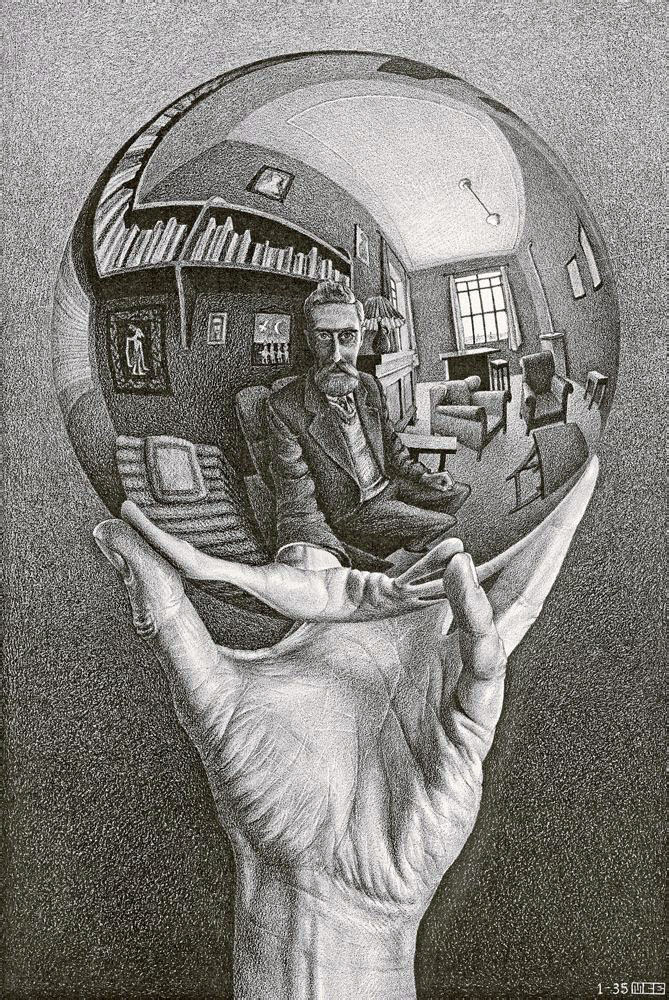
\includegraphics[height=.9\textheight]{img_007.jpg}
\caption[拿着反光球的手,艾舍尔作。]
  {举着反光球的手。毛里茨·康奈利斯·艾舍尔的自画像(蚀版画,l935)。}
\end{figure}

怪圈概念中所隐含的是无穷概念。循环不就是一种以有穷的方式表示无休止过程的方法吗?无穷在艾舍尔的许多画中起着重要作用。同一主题的许多副本常常扣在一起,构成对应于巴赫卡农的视觉形象。艾舍尔著名的版画《变形》(\fig{8})中就有好几个这样的图案。它有点像“无穷升高的卡农”:先是离开起点越来越远,然后突然回来了。《变形》以及别的画中的贴着瓷砖的平面已经暗示出了无穷。但是艾舍尔其它的画把无穷表现得更强烈。在他的一些画中,一个单一主题可以出现在现实的不同层次上。比如,某幅画中的一个层次可以被清楚地看作是在表现幻想或想象,另一个层次则会被认为是表现现实。这两个层次可能是仅有的明确地画出来的层次。但是单这两个层次便使观者不由得把自己看成是另外一个层次的一部分,这样一来,这位观众就不由自主地被艾舍尔画中隐含的层次串所俘获了。在这个串中,对于任何一个层次来说,在它之上都有另一个层次比它更为“实在”,同样,也总有一个在它之下的层次比它更为“虚幻”。单是这一点已足以让人头疼了。但如果这个层次串不是直线的,而是形成了一个圈,又将发生什么呢?那时候什么是实在的?什么是虚幻的?艾舍尔的天才在于,他不只是能设想出,而且还实际画出了几十种半实在半虚幻的世界,几十种充满了怪圈的世界,他似乎正在邀请他的观众们走进这些怪圈中去。

\begin{sidewaysfigure}
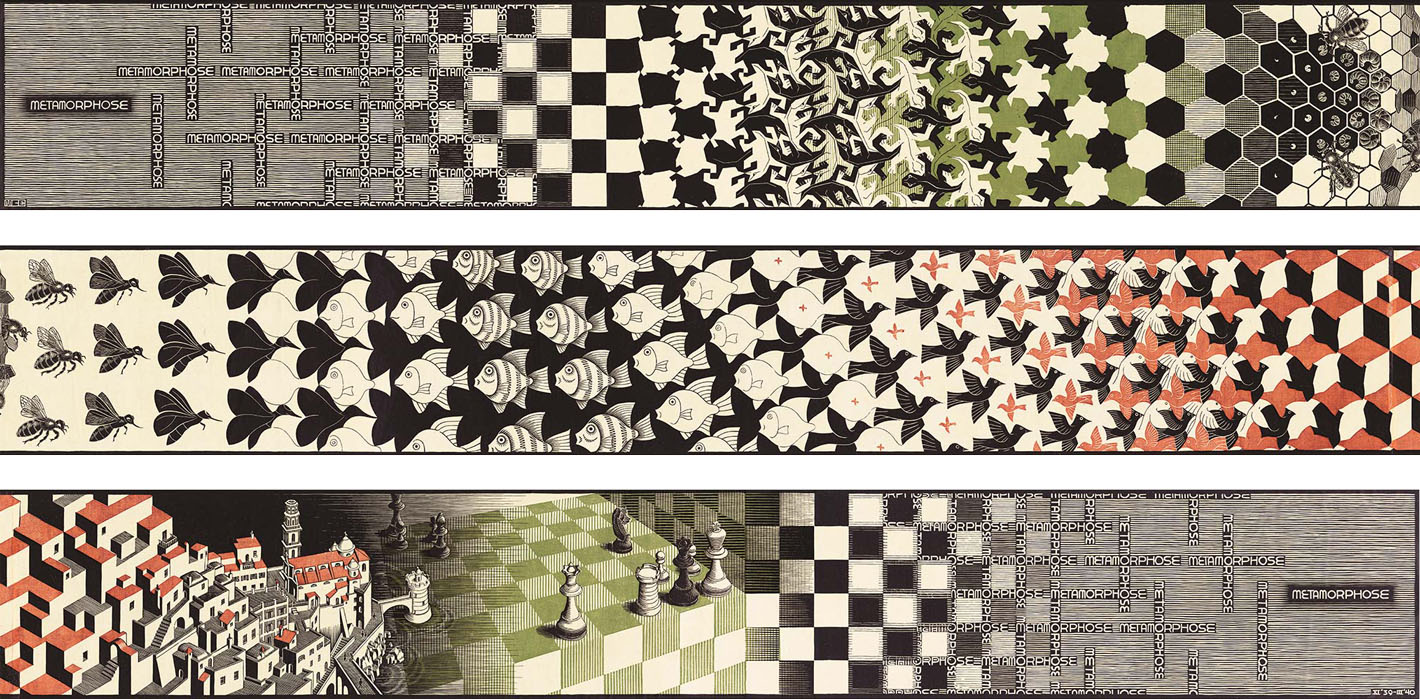
\includegraphics{img_008.jpg}
\caption[变形II,艾舍尔作。]
  {变形II,艾舍尔作(木刻,$19.5\times400$厘米,1939--1940)。}
\end{sidewaysfigure}

\section{哥德尔}

\begin{figure}
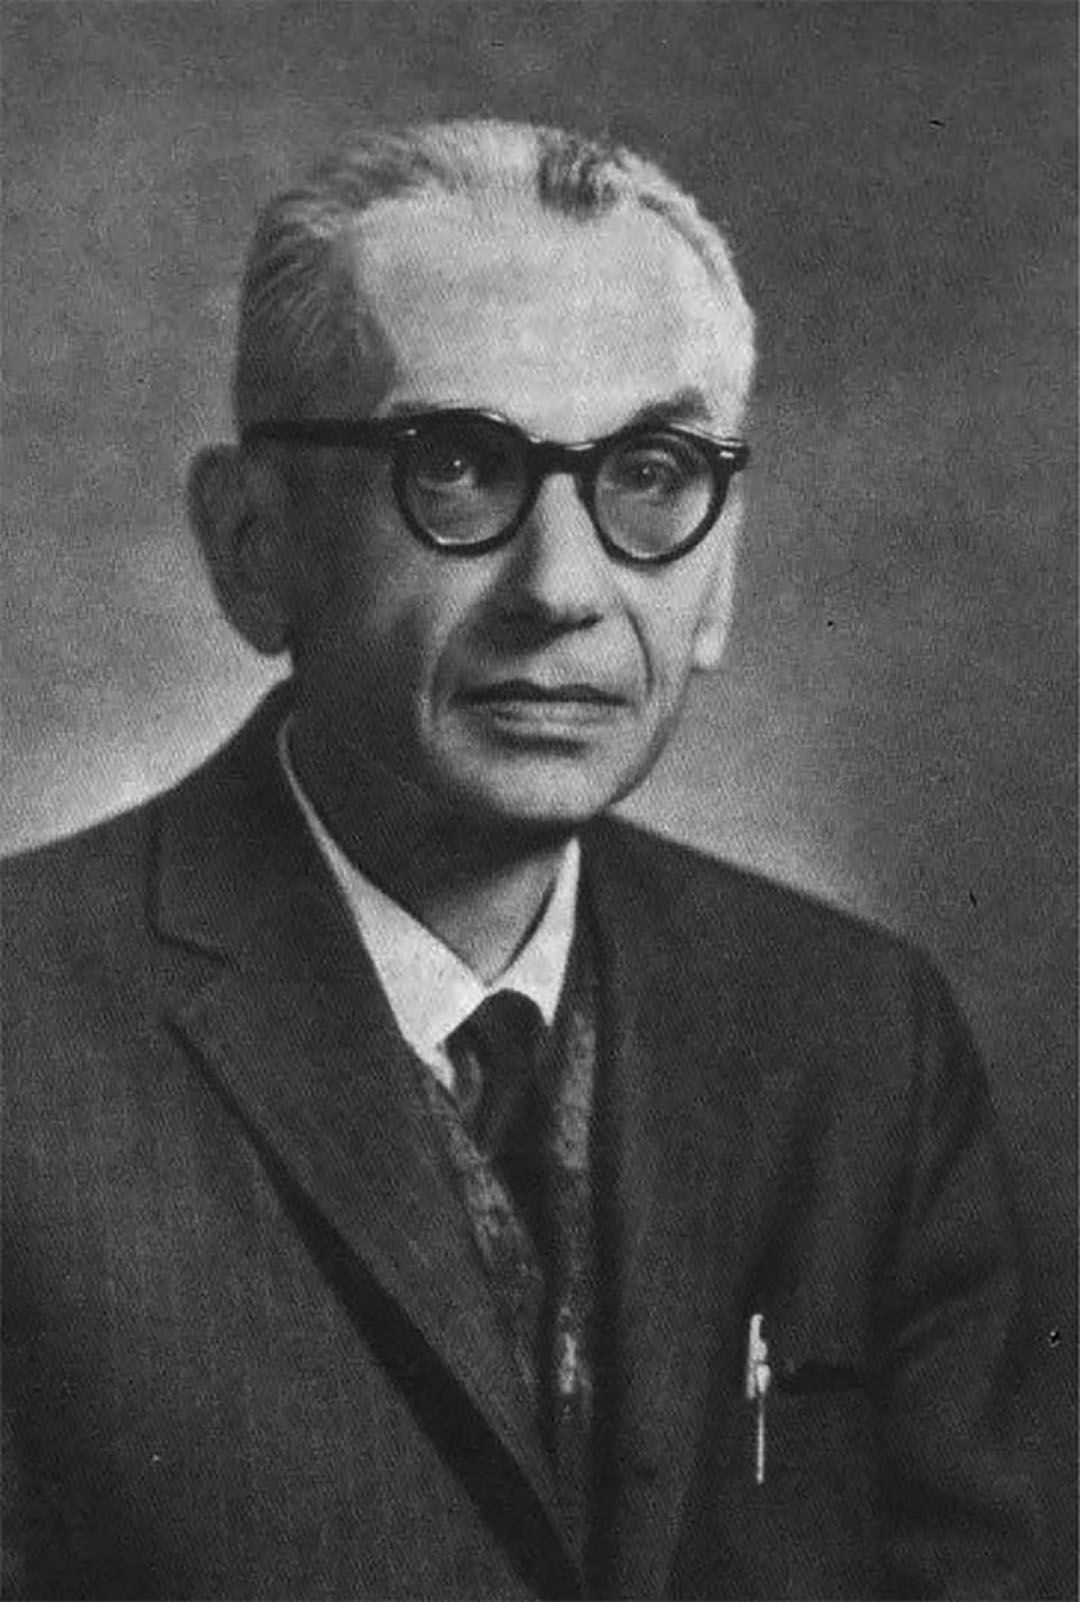
\includegraphics[height=.8\textheight]{img_009.jpg}
\caption{库特·哥德尔。}
\end{figure}

在我们看到的巴赫和艾舍尔的怪圈例子中,存在着有穷与无穷之间的冲突,因而使人有一种强烈的悖论感。我们直觉到这里面涉及到了什么数学问题。二十世纪确实发现了一个产生了巨大反响的数学上的对应物。正像巴赫和艾舍尔的圈是作用于人们简单而古老的直观一样(音阶和楼梯),哥德尔对数学系统中怪圈的发现,也有着它简单而古老的直观根源。就其最简单的形式而言,哥德尔的发现涉及到把一个古老的哲学悖论转化成数学上的说法。那个悖论就是所谓的“艾皮曼尼蒂斯悖论”,即“说谎者悖论”。艾皮曼尼蒂斯是一个克里特岛人,他说过一句不朽的话:“所有克里特岛人都是说谎者。”这一语句的一种更直截了当的说法是:“我在说谎”,或者,“本句子是假的”\note{译者注:从前,人们认为这两个陈述都是悖论,而二十世纪罗素指出了前者不是悖论。因为由前者的真可以推出它假,而由前者的假则不能推出它真。}。我说的艾皮曼尼蒂斯悖论在本书中通常是指最后那个说法。这个陈述粗暴地违反了通常设定的把陈述分为真与假的二分法。因为,如果你假定它是真的,那么它会立即产生相反的结果,使你认为它是假的。但是,如果你假定它是假的,同样会产生相反的结果,让你又回到它必须是真的这一点上。你可以试试看!

艾皮曼尼蒂斯悖论是一个一步的怪圈,就像艾舍尔的《画廊》一样。但是它与数学有什么关系呢?这正是哥德尔所发现的。他的想法是用数学推论探索数学推论本身。这种使数学“内省”的观念有巨大的威力,也许它最丰富的涵义就体现为哥德尔发现的\emph{哥德尔不完全性定理}。这个\emph{定理}说了些什么与它如何被证明是两件不同的事情。我们将在本书中讨论有关这两件事的详细情况。可以把这一\emph{定理}比做是一颗珍珠,而证明它的方法则是一只牡蛎。珍珠由于它的光泽和朴素而被称赞,牡蛎则是一个复杂的有生命的动物,它的内部结构是产生这种神秘的小珍宝的根由。

\emph{哥德尔定理}是作为他一九三一年的一篇论文中的命题VI而出现的,这篇论文的题目是:“论《数学原理》及有关系统中形式上不可判定的命题I”。该命题是这样叙述的:

\begin{quote}[]
对公式的每个$\omega$一致的递归类$\kappa$,对应着一个递归的类记号$\gamma$,使得$\nu\operatorname{Gen}\gamma$或$\operatorname{Neg}(\nu\operatorname{Gen}\gamma)$都不属于$\operatorname{Flg}(\kappa)$(其中$\nu$是$\gamma$的自由变量)。
\end{quote}
原文是德文,也许你觉得这种表达无论如何仍是德语式的。所以这里用更易懂的汉语把它改写为:

\begin{quote}[]
数论的所有一致的公理化形式系统都包含有不可判定的命题。
\end{quote}
这就是那颗珍珠。

在这颗珍珠里很难看到怪圈。这是因为怪圈被埋藏在牡蛎——证明之中了。哥德尔不完全性定理的证明的关键在于能写出一个自指的数学陈述,就像说谎者悖论是语言中的自指语句一样。尽管用语言来谈论语言似乎是很简单的,然而,要发现如何让一个关于数的陈述能够谈论它自身,可就不那么容易了。事实上,只有天才才能将自指陈述的概念与数论联系起来。哥德尔一旦通过直觉发现这样一种陈述是可以创造出来的,他就已经跨越了主要障碍。这一陈述的实际创造就是这一优美的直觉火花所产生的结果。

在以后的章节中,我们将仔细研究哥德尔的建构。但是为了不致使读者现在完全不知所云,我将在这里概略地描画一下它的概念核心,希望能够对读者有所启发。首先要把难点彻底弄清楚。数学陈述——这里我们只讲数论的陈述——是关于整数的性质的。整数不是陈述,也不是它们的性质。一个数论陈述不是关于数论陈述的,它仅仅是一个数论陈述,这就是问题所在。但是哥德尔认识到还有比眼前更多的东西。

哥德尔洞察到,只要数能够用来代表陈述,那么一个数论陈述就可以是关于一个数论陈述的了(甚至可以是关于它本身的)。换句话说,编码的概念是哥德尔构造的核心部分。在哥德尔编码——通常称做“哥德尔配数”——中,数是用来代表符号和符号序列的。这样,每个数论陈述作为一个特定的符号序列,获得了一个可资查询的哥德尔数,这有点像电话号码或行车执照。这种编码方式可以使人们从两个不同的层次去理解数论陈述:把它理解成数论陈述,同时也可以理解成关于数论陈述的陈述。

哥德尔一旦发明了这种编码的方法,他就得找出一个具体的把说谎者悖论转换成数论形式的方法。他最后移植的说谎者并不是说:“本数论语句是假的”,而是说:“本数论陈述是不可证的”。这可能会引起极大的混乱,因为人们通常对于“证明”这一概念理解得很模糊。哥德尔的工作实际上正是数学家们力图澄清什么是证明这一长期努力的一部分。要记住的重要事情是,证明是在确定的命题系统范围内的论证。在哥德尔的工作中,“证明”一词所涉及的那个特定的数论推理系统,就是1910至1913年间出版的罗素和怀特海合著的巨作《数学原理》中的那个系统。因此,哥德尔句子G写成下列的汉语陈述更为合适:

\begin{quote}[]
这个数论语句在《数学原理》的系统中是不可证的。
\end{quote}
顺便提一句,哥德尔句子G不是哥德尔定理——就像说谎者句子不是“说谎者句子是一个悖论”这一结论一样。现在我们可以来谈谈发现了G会产生什么效果了。说谎者句子构成了一个悖论,因为它既不是真的又不是假的,而哥德尔句子G是一个(在《数学原理》中)不可证的但却是真的句子。结果呢?《数学原理》中的系统是“不完全的”——存在有真的数论陈述,但系统的证明方法太弱,以致于无法证明它。

《数学原理》是这一打击的第一个牺牲品,但绝不是最后一个。哥德尔那篇论文的标题中的“及有关系统”这几个字,蕴涵着丰富的潜在内容。因为假如哥德尔的结果仅仅是指出了罗素和怀特海书中的一个缺陷,那么其他人可能会得到启发,并对《数学原理》作出改进,从而比\emph{哥德尔定理}更胜一筹。但这是不可能的:哥德尔的证明适用于任何一个企图达到怀特海和罗素为自己所设立的那个目标的公理系统。对于各种不同的系统,都有一个基本的方法变出这一戏法。简而言之,哥德尔展示了,无论涉及到什么公理系统,可证性总是比真理性弱的概念。

因此,\emph{哥德尔定理}对于那些对数学的基础感兴趣的逻辑学家、数学家和哲学家们产生了震撼性的影响。因为它展示出了,无论多么复杂的确定的系统,都不能表示出整数:$0$, $1$, $2$, $3$, \ldots\ 的复杂性。今天的读者也许不会像一九三一年时的读者那样为此而困窘。这是因为这期间我们的文化已经把\emph{哥德尔定理}连同相对论和量子力学等观念上的革命一起吸收了。与此相关的那些令人困惑的哲学观点尽管几经转述也早已为大众所知(通常是多一层转述,多一分困惑)。如今普遍存在着一种可以料想“限制性”结果的心理——但在一九三一年,它简直像是晴天霹雳。

\section{数理逻辑:一份提要}

要想真正领略\emph{哥德尔定理}的风采,需要一整套背景。因此我要在这里用很小的篇幅总结一下1931年以前的数理逻辑史——这是一种几乎不可能的工作。(参看德朗[DeLong],尼朋[Kneebone]或纳格尔[Nagel]与纽曼[Newman]合著的著作,它们都是很好的关于数理逻辑史的书)。事情是从将推理的思维过程加以机械化这一努力开始的。通常认为,使人类有别于其它动物的东西就在于人类有推理能力。所以把最代表人类特点的东西加以机械化,这乍看起来多少有点自相矛盾。然而,即使是古代希腊人也懂得推理是种合乎一定规范的过程,起码是部分地受固定的规律支配的。亚里士多德把三段论规范化,欧几里德整理了几何学,但是自那以后过了许多世纪对公理化推理的研究才又有所进展。

十九世纪数学上一个意义深远的发现是人们认识到存在着几种不同的,但却是同等有效的几何学——这里所说的“几何学”是指关于抽象的点与线的性质的理论。长期以来,人们认为几何学就是欧几里德所编纂的那个样子。虽然欧几里德的表述可能有小的错误,但那是无关紧要的。几何学上任何真正的发展都只有通过对欧几里德几何学加以扩充才能获得。这一观念被若干人几乎是同时地对非欧几何学的发现给摧毁了——这一发现震动了数学界,因为它对于“数学是研究现实世界的”这种观念提出了深刻的挑战。在单一的现实里如何能存在着不同种类的“点”和“线”呢?如今,这一问题的答案是显而易见的,甚至对于一些非数学家来说也不困难。但是,在那个时候,这一难题在数学界造成了混乱。

十九世纪晚期,英国逻辑学家乔治·布尔和奥古斯都·德·摩根比亚里士多德进了一大步,整理出了严格的演绎推理模式。布尔甚至把他的书命名为《思维的法则》,这当然是夸张,但是它确实是一项重大的贡献。刘易斯·卡罗尔迷上了这些机械化的推理方法,并且发明了许多可以用这些方法解决的谜题。耶那的高特洛布·弗雷格和都灵的朱瑟佩·皮亚诺进行着将形式推理与对集合与数的研究结合起来的工作。哥廷根的大卫·希尔伯特则致力于对几何学进行比欧几里德更为严格的形式化。所有这些努力都指向了对人们所说的“证明”是什么含义这一问题的廓清。

与此同时,古典数学也有了有趣的进展。十九世纪八十年代,盖奥尔格·康托尔发展了关于各不同类型的无穷的理论,也就是人们所知道的集合论。这个理论是有力的、优美的,但是很不直观。不久以后,各种各样的集合论悖论就被发现了。当时的形势十分令人困惑,因为正当数学似乎就要从一批悖论(即微积分中与极限理论有关的悖论)中摆脱出来的时候,又出现了一大批新的、看起来更糟糕的悖论。

其中最著名的是罗素悖论。大多数的集合,看起来不会是它们本身的元素——例如,海象的集合不是一只海象,由圣女贞德一个人组成的一个集合并不等于圣女贞德本人(一个集合不是一个人),诸如此类。从这一点看来,大多数集合是“普通的”。然而,有些“自吞”的集合确实包括其自身作为该集合的元素。例如包括所有集合的集合,或包括除圣女贞德之外的一切事物的集合等等。显然,每一个集合不是普通的便是自吞的。不可能有一个集合是兼而有之的。现在,没有什么能阻止我们发明一个$\mathscr R$:一个包括所有普通集合的集合,乍看起来,$\mathscr R$似乎是一个相当普通的发明,但是,你一旦问自己:“$\mathscr R$本身是一个普通的集合还是一个自吞的集合?”原来的看法就必须修正了。你会发现答案是:“$\mathscr R$既不是普通的也不是自吞的集合,因为任何一个选择都将导致悖论。”不妨试试看!

但是如果$\mathscr R$既不是普通的又不是自吞的集合,那么它是什么呢?最起码,它是病态的。但是谁也不会对这种遁辞式的回答满意。于是人们开始更深地探讨数论的基础。关键问题似乎在于:“我们对于‘集合’的直观概念有什么毛病?我们能够构造与我们的直观很相符但又可以绕过悖论的严格的集合论吗?”就像在数论和几何学那里一样,此处的问题是要试图把直观与形式化的或公理化的推理系统协调起来。

我们还可以构造一个令人吃惊的罗素悖论的变种,名为“格瑞林悖论”,它可以使用形容词而不是集合来形成。先把汉语中的形容词分成两类:一类是自描述的,像“四个字的”,“糟糕至极的”和“寡乎稀然的”;另一类是非自描述的,像“可以吃的”,“不完全的”和“两个音节的”。现在,假如我们承认“非自描述的”这个词是一个形容词,那么它属于上面的哪一类呢?我们可以为这一悖论发明两个词:自谓的($=$“自描述的”),和非自谓的($=$“非自描述的”)。这样一来,问题就变成了:“‘非自谓的’这个词是非自谓的吗?”试试看!

这些悖论有一个共同的祸根,就是自指,或称“怪圈”。所以,如果目的在于取缔一切悖论,为什么不去取缔自指以及一切允许产生自指的东西呢?这看起来容易,其实不然。因为要断定自指出现在什么地方是非常困难的。一个怪圈可能会在好几个步骤中才能完全展开,就像下面这个“扩展了的”说谎者悖论,它使人联想起《画手》:

\begin{center}
下面这个句子是假的。\\
上面那个句子是真的。
 \end{center}

放在一起看,这两个句子和原来的说谎者悖论有着同样的效果。但是分开来看,它们却是无害的、甚至很可能是有用的句子。这个怪圈不能“归咎”于任何一个句子,而应归咎于它们互“指”对方的方式。同样,在《上升与下降》这幅画中,每个局部都是合理的,只是把它们组合在一起,才出现了不可能的事。由于有间接的和直接的两种自指,必须断定如何同时取缔两者——如果把自指看成是万恶之源的话。

\section{消除怪圈}

罗素和怀特海是赞成这一观点的。因此,《数学原理》就是从逻辑学、集合论和数论中驱除怪圈的一次庞大实践。他们的系统的基本点是这样的:有一个“类型”最低的集合,只能包含“对象”而不是集合做元素。高一层类型的集合,只能包含对象或最低类型的集合。一般的说,一个给定类型的集合只能包含对象或类型低于它的集合。每一个集合都属于一个特定的类型。很清楚,没有一个集合可以包含自己,因为,包含它的集合得属于比它更高的类型。在这样的系统中只能有“普通的”集合。此外,前面提到的$\mathscr R$——所有普通的集合的集合——不再被看作是一个集合了,因为它不属于任何一个有穷类型。于是,整个看来,这种类型论——我们也可以把它叫做“取缔怪圈的理论”——成功地摆脱了集合论的悖论,但是这是以引进看起来是人为的层次为代价的,并且不允许形成某些类的集合,比如所有普通集合的集合。从直观上说,我们并不是这样来设想集合的。

类型论解决了罗素悖论,但对于说谎者悖论或格瑞林悖论却不起作用。对于那些兴趣不超出集合论的人来说,这已经足够了——但是对于想消除一般悖论的人,就必须有一些类似的“分层法”来禁止语言中的循环。在这个层次结构的最底层是对象语言。对象语言只涉及特定的域,而不涉及对象语言本身(比如它们的文法规则,或其中的具体句子)。如要涉及它们,则要有一种元语言。对于语言的两个层次这一经验,所有学习外国语的人都是很熟悉的。然后,就要有一种元元语言来讨论元语言,以此类推。这就要求每一个句子都明确属于层次结构的某一层。那么,如果一个给出的句子找不出它属于哪一层,这个句子就会被认为是无意义的,因而被忘掉。

现在可以尝试来分析上面给出的说谎者的两步循环。第一个句子,因为它谈论第二个句子,所以一定比第二个句子高一层。但是,根据同样的道理,第二个句子一定比第一个句子高一层。由于这是不可能的,所以两个句子都是“无意义的”。更准确地说,这样的句子根本不可能在建立于严格语言层次上的系统中形成。这样就防止了任何样式的说谎者悖论以及格瑞林悖论。(“非自谓的”属于哪一语言层?)

在集合论中,研究的都是些不常用到的抽象对象,像类型论那样的分层,尽管有点古怪,还是可以接受的。但是如果涉及的是语言,是渗透于生活各处的语言,这种分层就显得荒唐了。我们在说各种不同的事物时,不会想到我们是在语言的层次间上蹿下跳。像这样的句子:“在本书中,我批评了类型论”,平平常常,却会在我们所讨论的系统中被双重禁止:第一,它提到了“本书”,而这是只能在“元书”中提及的东西;第二,它提到了“我”,而这是我这个人所根本不允许提到的一个人!这个例子指出,当你把类型论引入一个你所熟悉的情景中时,它看上去是多么愚蠢。我们采用的补救悖论的办法——把任何形式的自指全部驱除——实际上是一种过头的做法,它把许多完美无缺的语言构造都算作是无意义的了。顺便提一下,“无意义的”这个形容词,必然会用于所有有关语言学类型理论的讨论(如本段的讨论)。因为很明显,这些议论不会出现在任何一层——不论是对象语言,还是元语言,或元元语言等等。因而,对这个理论进行讨论这一行动本身,就构成了对此理论所有可能的违背之中最明目张胆的一个!

有的人可能要为这些理论辩护,理由是它们只打算处理形式语言,而不打算涉及日常的、非形式的语言。可能是这样,但是它说明这些理论是极端经院式的,而且对于悖论并没有说什么,除非是在特别造出来的系统中所产生的悖论。另外,这种不惜一切代价消除悖论的做法,尤其是当它需要创造人为的形式系统的时候,未免就太过于强调简单的一致性,而忽视了离奇与怪异,而正是后者才使得生活与数学趣味无穷。当然,保持一致性很重要。但是这种努力如果迫使你进入一个非常丑陋的理论,你就会觉得什么地方出毛病了。

数学基础中的这类问题使人们对出现于二十世纪早期的将推理方法规范化的尝试抱有浓厚的兴趣。数学家和哲学家开始产生重大的怀疑:即使是最具体的理论——如整数研究(数论)——是否已建立在坚实的基础之上?如果悖论能那么轻易地出现于集合论——一个其基本概念,即集合,在直观上如此吸引人的理论——之中,那么其它的数学分支不也可能有悖论吗?另外一个与此有关的担忧是逻辑的悖论,像说谎者悖论,它们很可能是数学中固有的。要是这样,全部数学就变得可疑了。这尤其使那些为数不少的坚信数学只是逻辑学的一部分(或者相反,逻辑学是数学的一部分)的人觉得忧心忡忡。事实上:“数学与逻辑学是否是有别的、分离的”这一问题,是很多争论的根源。

对于数学本身的研究被称为元数学——或者有时被称为元逻辑,因为数学与逻辑是如此紧密地相互交织在一起的。元数学家最紧要优先考虑的事情是决定数学推理的真正性质。什么样的推理手段是合法的?什么样的是不合法的?由于数学推理使用的都是“自然语言”,(如法语、拉丁语或用于通常交流的其它语言),因此总是有许多可能的歧义,可以唤起不同的意象等等。看起来,建立一套统一的记号是合理甚至是重要的。用这种记号可以做一切数学方面的工作,通过使用这种记号,可以帮助任何两个数学家解决提出的某个证明是否有效这样的争论。这样,就需要一套完整的关于普遍公认的人类推理模式的法典,至少用于数学推理时是这样。

\section{一致性、完全性和希尔伯特方案}

企图从逻辑学中导出所有的数学,而且一定不能有矛盾,这就是《数学原理》一书要达到的目的。这本书受到普遍赞赏,但是没有一个人肯定:\pnum{1}是否一切数学都包括在罗素和怀特海所勾画的方法之中;\pnum{2}甚至不能肯定,这些给出的方法是否自身是一致的。不论是什么样的数学家,只要是按照罗素和怀特海的方法去做的,就永远不会得出矛盾的结果,这一点是绝对清楚的吗?

这个问题尤其困扰着著名的德国数学家(也是元数学家)大卫·希尔伯特。他曾向世界上的数学家(和元数学家)提出这样一个挑战:严格地论证(可能就是用罗素与怀特海提出的方法)《数学原理》一书中定义的系统既是一致的(无矛盾的)又是完全的(也就是说:每一个数论的真陈述都可以在《数学原理》所给出的框架之中推导出来)。这是一个很高的要求,人们可以批评它多少有点循环论证:你如何能用你的推理方法来证明你所用的这一套推理方法是正确的呢?这就好像是要拽着自己的鞋带把自己举起来。(我们好像简直无法从这些怪圈中解脱出来!)

希尔伯特当然充分了解这种两难局面。因而表示希望找出一个对一致性或完全性的论证,而这个论证只用到推理的“有穷”形式,即那些通常被数学家所接受的一小类推理方法。希尔伯特希望,用这种方法,数学家们可以拽着自己的鞋带把自己部分地举起来:只利用数学中的一小部分方法来证明整个数学方法是正确的。这一目的听起来也许很渺茫,但是它在二十世纪的前三十年占据了世界上许多最伟大的数学家们的思想。

但是,在1931年,哥德尔发表了他的论文,这篇论文从某种角度讲彻底粉碎了希尔伯特方案。它揭示了不仅在罗素和怀特海提出的公理系统中有不可弥补的“漏洞”,并且,更一般地说,没有一个公理系统可以产生所有的数论真理,除非它是一个不一致的系统!最后,要证明一个像《数学原理》中提出的那种系统的一致性是徒劳的:如果能只使用《数学原理》里边的方法找到这样一个证明的话,那么,《数学原理》本身就将是不一致的!——这是哥德尔的工作中那些最使人感到神秘的结论之一。

最大的讽刺是,\emph{哥德尔不完全性定理}的证明涉及到要把艾皮曼尼蒂斯悖论引进到《数学原理》的核心中,而《数学原理》原本被认为是一座完全可以抵御怪圈侵袭的堡垒!虽然哥德尔的怪圈没有摧毁《数学原理》,但却使数学家们对它的兴趣大大地减小了,因为哥德尔指出,罗素和怀特海原来的目的是一种幻想。

\section{巴比奇、计算机、人工智能…}

哥德尔的论文发表之际,世界正处在发展电子数字计算机的前夕。那时关于机械的计算机器的想法已经出现了有一些时候了。十七世纪,帕斯卡和莱布尼茨设计了进行固定运算(加法和乘法)的机器。不过,这些机器没有存储器,用现在的术语来说,它不是可编程序的。

第一个构想出这种有巨大计算潜力的机器的人是个伦敦人,查尔斯·巴比奇(1792--1871),一个几乎像是从《匹克威克外传》中走出来的人物。巴比奇生前因为发起了一场让伦敦摆脱“街头讨厌的事”——主要是那些手摇风琴师——的运动而大名鼎鼎。那些喜欢惹他发火的讨厌的家伙,常常不分白天黑夜前来演奏小夜曲,于是他便火冒三丈地在街上驱赶他们。今天,我们公认他是一位超前了他的时代一百多年的人物:他不仅是现代计算机原理的发明者,而且还是第一个向噪音污染做斗争的人。

他的第一部机器“差分机”,可以用“差分法”算出许多种类的数学表。但是在制造出任何“差分机”模型之前,巴比奇迷恋上了一个更具有革命性的想法:那就是他的“分析机”。他相当不谦虚地写道:\quotetext{“我发明分析机的思维过程大概是人类曾经有过的最复杂和最令人困扰的历程。”}\note{查尔斯·巴比奇,《一位哲学家生活中的片段》,第145--146页。}同以前设计的机器不同,这种“分析机”带有存储器(记忆器)和“加工装置”(计算和做出判定的部件)。这些部件是把许许多多个复杂的带齿的圆柱形装置用令人难以置信的复杂方式啮合在一起。在巴比奇的想象中,数字打着转在加工装置里进进出出,受控于穿孔卡片中的程序——这一想法来自雅卡提花机的启发,那是一种卡片控制的提花机,能织出惊人复杂的图案。巴比奇有一个出众的但命途多舛的朋友,女伯爵艾达·洛芙莱丝命妇(拜伦勋爵的女儿),她曾经富有诗意地评论说:\quotetext{“恰似雅卡提花机织出花朵和枝叶一般,分析机正织出代数的图案。”}不幸的是,她错用了“正”字,因为那时还未造出分析机,巴比奇是怀着痛苦的失望辞世的。

洛芙莱丝命妇和巴比奇一样,深深地意识到随着分析机的发明,人类将可以产生机械化的智能。尤其是如果它能“自食其尾”(这是巴比奇用以描述当一部机器探进自己的内部,改变它内部所存储的程序时所产生的怪圈的说法)的话。在1842年的回忆录中她写道\note{洛芙莱丝命妇为梅那布雷阿[Menabrea]所著的回忆录《查尔斯·巴比奇发明的分析机草案》所作的注释,日内瓦,1842年版。重印收入P.和E.莫里森[P. and E. Morrison]合著的《查尔斯·巴比奇和他的计算机械》[\bn{Charles Babbage and His Calculating Engines}],第248--249页。}:\quotetext{“\lnote{(分析机)}除了数值的计算之外,可以进行其它的计算”}。当巴比奇梦想着发明一种能下棋或玩九格棋游戏的自动机时,她建议把一个个的音与和弦编入他机器的旋转圆柱体中,\quotetext{“这样就可以创作出精美的、符合科学的、要多复杂就有多复杂的曲子。”}但是几乎在同时,她告诫道:\quotetext{“分析机没有创造性。它只会做我们知道如何去命令它执行的事情。”}虽然她非常理解人工计算的力量,洛芙莱丝命妇对于人工生成智能是持怀疑态度的。但是,她深刻的洞察力允许她去梦想人类对电的驯服所能开发出的潜力吗?

到我们二十世纪,制造计算机的时代已经成熟,这些计算机超过了帕斯卡、莱布尼茨、巴比奇或洛芙莱丝命妇最大胆的梦想中的计算机。在二十世纪三十年代和四十年代,第一批“大电脑”被设计并制造出来了。它把原来彼此独立的三个领域综合在一起了。这三个领域是:关于公理化推理的理论、机械计算的研究和智能心理学。

这些年同样是计算机理论日新月异的年代。这些理论与数学有紧密的联系。事实上,\emph{哥德尔定理}在计算理论中有其对应物,这是阿兰·图灵发现的。它揭示出了即便是在可以设想出来的性能最好的计算机中,也存在有不可避免的“漏洞”。带有讽剌意味的是,正当这些怪异的局限性被发现的时候,不断造出的真正的计算机的性能却越来越好,远远超出了他们的制造者的预见力。巴比奇曾经说过,假如他能在五百年后回到世界上进行一次为期三天的有向导的科学旅行,他将很愿意放弃他的余生。在他去世后仅一百年的今天,如果他能回来,看到当今新的机器以及它们出人意料的局限性,他会惊奇得说不出话来。

五十年代初期,机械化智能似乎已指日可待了,然而,在创造最终的真正的思维机器时,每跨跃一个障碍都要产生一个新的障碍。目标的这种神秘的退避有什么深刻的原因吗?

谁也不知道非智能行为和智能行为之间的界限在哪里。事实上,认为存在明显界限也许是愚蠢的。但是智能的基本能力还是确定的,它们是:
\begin{itemize}
\item 对于情境有很灵活的反应;
\item 充分利用机遇;
\item 弄懂含糊不清或彼此矛盾的信息;
\item 认识到一个情境中什么是重要的因素,什么是次要的;
\item 在存在差异的情景之间能发现它们的相似处;
\item 从那些由相似之处联系在一起的事物中找出差别;
\item 用旧的概念综合出新的概念,把它们用新的方法组合起来;
\item 提出全新的观念。
\end{itemize}

这里遇到了看起来像是悖论的东西。计算机的本性恰恰就是极不灵活、没有欲望、照章办事。尽管它们可能是速度很快的,它们仍然是无意识的东西。那么,如何能给需要智力的行为编出程序呢?这不是最最明显的自相矛盾吗?本书的一个主要论题就是讲这里根本不存在矛盾。本书的一个主要目的就是鼓励每一个读者,直接了当地面对这个表面上看来是矛盾的东西,尝一尝它的滋味,摆弄摆弄,拆开来看看,沉浸于其中,以使读者最终得以重新认识存在于形式化的和非形式化的、有生命的和无生命的、灵活的和不灵活的事物之间的那些表面上看来不可逾越的鸿沟。

这便是人工智能所要研究的全部。人工智能工作的奇异之处就是试图将一长串严格形式化的规则放在一起,用这些规则教给不灵活的机器如何能灵活起来。

但是什么样的“规则”可能把握住我们想到的所有的智能行为呢?当然,一定是在各个不同的层次上有不同的规则。一定有许多“十分平常的”规则,一定有“元规则”修改“十分平常的”规则,而且有“元元规则”修改元规则,等等。智能的灵活性来自大量的不同规则和规则的层次。之所以一定有许许多多的在不同层次上的规则,是因为在生活中,生物面对着成千上万的完全不同类型的境况。在某些境况中,只存在要求“十分平常的”规则的刻板反应。有些境况是一些刻板境况的混合——这样,就需要决定要使用哪些“十分平常的”规则的规则。有些境况无法分类——那么,就一定要有发明新规则的规则……等等。无疑,包含着那些直接或间接地改变自己的规则的怪圈是智能的核心。有的时候人类思维的复杂性看起来是如此的巨大,以致于人们觉得对于“理解智能”这个问题没有什么解决办法——人们觉得无法设想有某种规则可以控制生物的行为,即便所用的“规则”具有上述意义上的“多层次”。

\section{…和巴赫}

1754年,巴赫死后四年,莱比锡的神学家约翰·米凯尔·施密特在一篇关于音乐与灵魂的论文中写下了下面一段值得注意的话:

\begin{quote}
几年前,从法国来的一篇报道中说,一个人制作了一个木偶,它可以用长笛演奏各种曲子。它会把长笛放在唇边,再把它拿下来,还能转眼珠等等。但是,还没有一个人发明过能思维、有欲望、会作曲或者哪怕能做类似事情的偶像。请任何一个想要进一步信服这一点的人仔细地看看上面赞扬过的巴赫的刻在铜板上的最后一支赋格曲吧,只是由于他双目失明,这部曲子才未能完成。请研究研究里面所包含的艺术,或让我们来看看一定会打动我们的东西——那更为精彩的赞美诗吧!那是他失明后口授,别人代笔写成的作品:《当我们身陷危难之时》(\bn{Wenn wir in höchsten Nöthen seyn})。我敢肯定,如果人们想要研究包含在其中的所有的美——更不用说如果他自己想要演奏,或是评论一下作者——他马上就需要有灵魂了。看到这一例子,唯物主义斗士们的所有理论都将威风扫地。\note{大卫和曼德尔,《巴赫读本》,第255--256页。}
\end{quote}

这里提到的第一流的唯物主义斗士很可能不是别人,而是于连·奥伏瓦·德·拉·梅特利——腓德烈大帝的宫廷哲学家,《人是机器》一书的作者,最杰出的唯物主义者。到现在已是两百年过去了,而赞同施密特的人与赞同拉梅特利的人之间的斗争仍在激烈地进行着。我希望在本书中对这一论战提出一些看法。

\section{“哥德尔、艾舍尔、巴赫”}

本书是以一种不同寻常的方式构成的:在对话和章节之间有一种对位。这样构造的目的是为了使我能够让一个新的概念出现两次:几乎每一个新概念都是首先以隐喻的形式出现在对话中,给出一组具体可见的意象,然后,在阅读接下来的那一章的时候,它们可以作为一种直观背景来衬托对这同一个概念的更为严肃和更为抽象的表述。在许多对话中,我在表面上谈论着一个想法,但是实际上是以稍稍隐蔽的方式在谈论着另一个想法。

本来,我的这些对话中只有两个主人公:阿基里斯和乌龟。他们是我用与刘易斯·卡罗尔同样的方式从爱利亚的芝诺那儿借来的。芝诺是公元前五世纪的人,悖论的发明者。他的悖论之一是一个寓言,阿基里斯和乌龟是寓言中的主角。在我第一篇对话《三部创意曲》里,我交代了芝诺搞出这“快活的一对”的创意。1895年,卡罗尔让阿基里斯和乌龟再现了,目的是要阐明他的关于无穷的新悖论。卡罗尔悖论——事实上应该比现在更广泛地被人所知——在本书中起着重要作用。它原来的题目是“乌龟说给阿基里斯的话”,在本书中它作为对话《二部创意曲》出现。

在我开始写这些对话时,不知怎么搞的,我把它们与音乐形式联系起来了。我不记得是怎么开的头,只记得有一天,我在一篇早些时候写下的对话的标题位置上写下了“赋格”二字,从那以后,这一想法就固定下来。最后,我决定以各种各样的方式使每一篇对话都仿照巴赫的一支曲子。这样做并不是不得体的。老巴赫自己就常常提醒他的学生们说,他们作品中的每个部分应该写成“好像是一些精心搭配的人在一起交谈一样”。我接受这一教诲比起巴赫的原意来也许更咬文嚼字了些,然而我希望我的结果忠实于他的原意。特别使我产生灵感的是巴赫作品中那些一次又一次地打动我的特征,这些东西在大卫和曼德尔在《巴赫读本》一书中有非常好的描述:

\begin{quote}
他的形式通常建立在各个片段的不同关系上。这些关系有的是使各个段落构成完整的统一体,还有的则是回归到单一的精心安排的主音,或仅仅是一个主题的暗示。由此而产生的格式通常是对称的,但并非必须如此。有的时候,不同片段之间的关系像缠结在一起的细线组成的迷宫,只有通过仔细的分析才能解开。然而,通常在初看或初听起来的时候,只有少数占主导地位的特点可以指引方向。随着研究的深入,人们会发现无穷无尽的微妙之处。人们永远不会不知所措地抓不着把巴赫的各个单独的创造结合在一起而形成的那个统一体。\note{大卫和曼德尔,《巴赫读本》,第40页。}
\end{quote}

我设法把\emph{哥德尔}、\emph{艾舍尔}、\emph{巴赫}这三块稀世之宝嵌为一体,\emph{集异璧之大成}。开始时我打算写一篇以\emph{哥德尔定理}为核心的文章。我当时以为它仅仅会是一本小册子。可是我的想法像球面一样扩展开来,不久就触及了巴赫和艾舍尔。我花了一些时间去想如何把这一联系写清楚,而不仅仅是让它作为我自己写这本书的推动力。但是最后,我认识到,对我来说,哥德尔和艾舍尔和巴赫只是某个奇妙的统一体在不同方向上的投影。我试图揭示这块在我奇\emph{异}的收\emph{集}过程中所发现的瑰\emph{璧},结果产生了这本书。

\end{intro}
